
\chapter{Introduction}
\label{ch-1}

\lipsum[2-4]

\begin{marginfigure}
	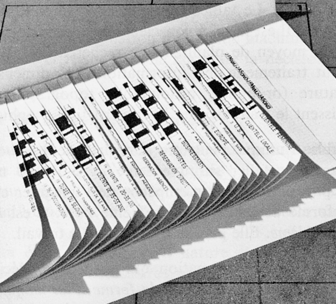
\includegraphics[width=\marginparwidth]{bertin_hotel}
	\caption[Matrices ré\-/ordonnables de Jacques Bertin.]{Matrices matériellement ré\-/ordonnables de  \citet{bertin_la_1977} utilisant une fiche par ligne, ce qui permet de reclasser manuellement les lignes par ré\-/agencement des fiches.}	
	\label{fig-bertin-matrice}
\end{marginfigure}

\lipsum[3]

\begin{figure*}[t]
	\centering
	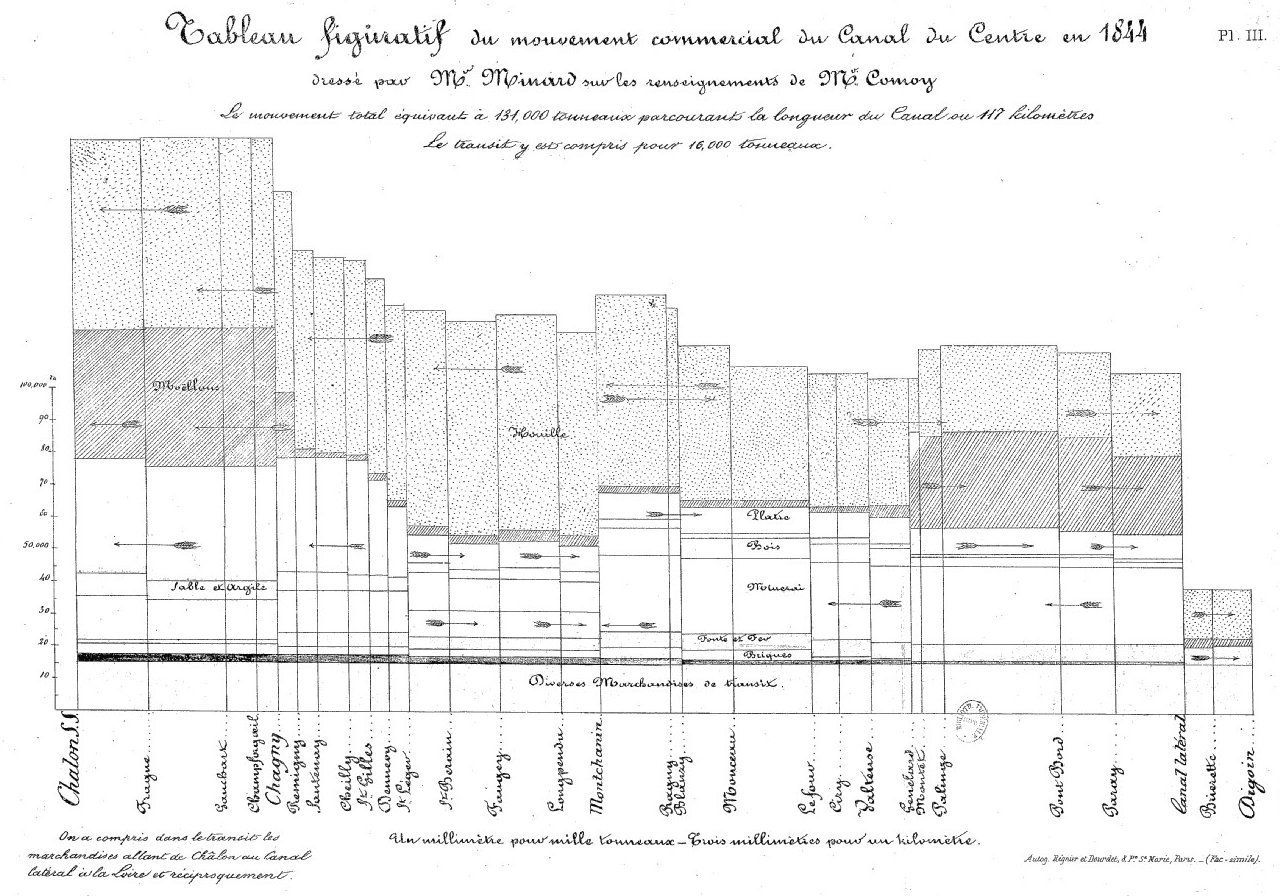
\includegraphics[width=\linewidth]{minard}
	\caption[Tableau graphique de Charles\-/Joseph Minard.]{Tableau graphique de Charles\-/Joseph Minard représentant le transport de marchandises sur le canal du Centre. La hauteur de chaque barre correspond à la charge (en nombre de tonneaux) et sa largeur à la distance de l'étape (en kilomètres), de sorte que l'aire représente le coût de transport (source: BnF~\citep{minard_des_1862}).}
	\label{fig-minard}
\end{figure*}

\lipsum[2]

\section*{Organisation du document}
Ce manuscrit de thèse est structuré en quatre chapitres principaux qui sont résumés dans les paragraphes suivant. 

Le \cref{ch-1} (\cpageref{ch-1}) \lipsum[1]

Le \cref{ch-2} (\cpageref{ch-2}) \lipsum[1]

\begin{margintable}
	\footnotesize
	\setlength\tabcolsep{.8pt} % default value: 6pt
	\begin{tabularx}{.95\marginparwidth}{Xl}
		\toprule
		& \thead{définition} \\
		\midrule
		{\faMobile*} & $ \approx 1-3$  \\
		{\faTablet*} & $ \approx 3-4$  \\
		{\faTv}   & $ \approx 2-8$ \\
		
		\bottomrule
	\end{tabularx}
	\caption{Définition standard des écrans de différents périphériques en millions de pixels.}
	\label{tab-ecrans}
\end{margintable}

Le manuscrit est ensuite conclu par un bilan et un résumé des perspectives de recherche envisagées avec calcul sur \gls{cpu}. L'\cref{ch-a} présente les détails des analyses statistiques des \glspl{trou_noir}.
